%%%%%%%%%%%%%%%%%%%%%%%%%%%%%%%%%%%%%%%%%%%%%%%%%%%%%%%%%%%%%%%%%%%%%%%%%%%%%%%%
\chapter{ИНТЕЛЛЕКТУАЛЬНЫЕ СИСТЕМЫ В ЗАДАЧАХ ФОРМИРОВАНИЯ ЦЕЛЕВОЙ РЕКЛАМЫ}
%%%%%%%%%%%%%%%%%%%%%%%%%%%%%%%%%%%%%%%%%%%%%%%%%%%%%%%%%%%%%%%%%%%%%%%%%%%%%%%%

Одной из задач данной работы является создание программного продукта, способного на основе клиентской базы данных генерировать события с рекламными сообщениями. Для решения такой задачи может быть использована  интеллектуальная система. Это следует из определения интеллектуальных систем и решаемых ими задач.

Интеллектуальная система (ИС) – это программный комплекс, который предназначен для решения задач различных типов в зависимости от потребностей пользователя. Интеллектуальная система в своей работе использует базу знаний и логико-математические средства для получения решения.

Интеллектуальная система способна решать различные задачи. Среди них: интерпретация данных, диагностика, мониторинг, проектирование, прогнозирование, планирование, обучение, управление, поддержка принятия решений и др~\cite{is1}.

В условиях данной работы, интеллектуальная система должна использовать базу знаний и логико-математические средства для решения задачи управления рассылкой рекламных сообщений.

Существуют разные типы интеллектуальных систем, каждая из которых более применима в той или иной ситуации. Для того чтобы понять, какая системы подходит для использования в таргетировании рекламы, необходимо рассмотреть различные типы интеллектуальных систем. Так же следует изучить вопрос устройства интеллектуальных систем. Это позволит разработать свой вариант ИС, применимый для решения поставленной задачи.

\section{Типы интеллектуальных систем и их характеристики}

Для интеллектуальных систем характерны такие свойства как развитая коммуникативная способность, умение решать плохо формализуемые задачи, способность к самообучению и адаптивности.

Коммуникативность ИС проявляется в способности взаимодействовать с конечным пользователем. Это позволяет ему формировать свои запросы для получения решения.

Решение плохо формализуемых задач определяется способностью ИС к построению оригинальных алгоритмов с возможностью использовать информацию о постоянно меняющихся данных и окружающей среде.
    
Самообучение заключается в возможности использовать накопленный опыт для решения новых задач.
    
Адаптивность позволяет системе подстраиваться под изменения модели проблемной области.
    
Исходя из перечисленных признаков можно разделить ИС на следующие типы:
    
\begin{itemize}
	\item системы с коммуникативными способностями (с интеллектуальным интерфейсом);
	\item экспертные системы (системы для решения сложных задач);
	\item самообучающиеся системы (системы, способные к самообучению);
	\item системы с адаптивными способностями.
\end{itemize}

Каждый из типов в свою очередь подразделяется на подтипы в зависимости от используемой технологии~\cite{is1}. Полная классификация представлена на рис.\ref{fig:ISTypes}.

\begin{figure}[H]
	\centering
	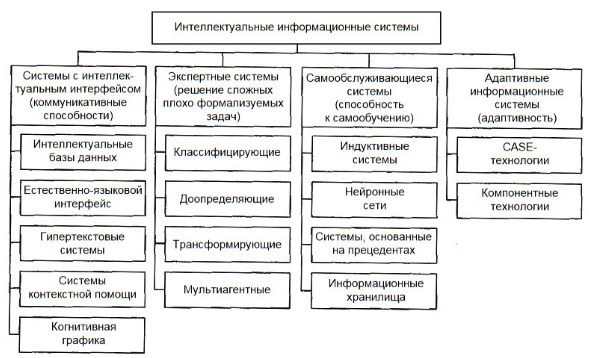
\includegraphics[width=\linewidth]{fig/ISTypes.jpg}
	\caption{Классификация интеллектуальных систем}%
	\label{fig:ISTypes}
\end{figure}

\textbf{Системы с интеллектуальным интерфейсом} направлены на улучшение способов взаимодействие с конечным пользователем.

\textit{Интеллектуальные базы данных.} Применяются для получения выборки данных, которая не хранилась БД в явном виде. В отличие от обычных БД выборка может быть сформирована на основе хранимой информации.

\textit{Естественно-языковой интерфейс.} Позволяет получать данные с помощью голосового ввода команд или машинного перевода с других языков. В работе таких систем используются модули морфологического, семантического и синтаксического анализа.

\textit{Гипертекстовые системы.} Используют метод поиска данных по ключевым словам. Работа такой системы происходит в два этапа. На первом из входных данных выделяются ключевые слова. На втором  обрабатывается информация извлеченная по выбранным ключевым словам.

\textit{Системы контекстной помощи.} При работе с такой системой пользователь описывает свой запрос, а система задает ему вопросы для конкретизации проблемы. На основе этой информации генерируется решение исходной задачи.

\textit{Системы когнитивной графики.} Используют графические образы для представления моделируемых и наблюдаемых процессов. Это позволяет пользователю легче воспринимать выводимую информацию и быстрее осваивать программный интерфейс интеллектуальной системы.

\textbf{Экспертные системы} создаются для частичной замены специалиста-эксперта в определенной области. Они позволяют формировать советы или принимать решения, основываясь на заранее записанном и формализованном опыте эксперта. Одним из важных качеств ЭС является возможность вывести ход своих рассуждений при принятии решения. 

\textbf{Самообучающиеся интеллектуальные системы} используют методы автоматической классификации ситуаций из реальных примеров. Примеры реализованы в обучающей выборке и для каждого из них сформированы ожидаемые критерии результата. В процессе обучения система сама генерирует правила, на основе которых способна классифицировать ту или иную исходную ситуацию. 

\textbf{Адаптивные информационные системы} применяются в областях, где исходные данные постоянно изменяются. Адаптивные системы отвечают двум специфическим требованиям:

\begin{itemize}
	\item способны отображать знания в каждый момент времени;
	\item пригодны для быстрой реконструкции при изменении проблемной среды.
\end{itemize}

Рассмотрев типы интеллектуальных систем, можно сделать вывод, что для решения задачи таргетирования рекламы подходит подтип экспертных системы, позволяющих управлять процессом генерации рекламных событий.

\section{Типовая структура экспертных систем}

Определившись с типом интеллектуальной системы, стоит рассмотреть ее типовую структуру. В дальнейшем, это позволит правильно спроектировать архитектуру программного приложения.

Экспертная система может быть двух видов: статическая и динамическая. Отличие динамической системы от статической в том, что она учитывает изменение знаний, которые могут произойти в процессе решения задачи.

В общем случае статическая ЭС состоит из 6 основных компонентов:
\begin{itemize}
	\item база знаний;
	\item база данных или рабочая память;
	\item решатель (интерпретатор);
	\item система объяснений; 
	\item компоненты приобретения знаний;
	\item интерфейс взаимодействия с пользователем. 
\end{itemize}

\textbf{База знаний} ЭС включает в себя данные, описывающие некоторую предметную область. База знаний, так же содержит правила, позволяющие производить логическое рассуждение и преобразовывать хранимые знания в решения поставленных задач.

\textbf{База данных (рабочая память)} содержит данные, используемые в решении текущей задачи.

\textbf{Решатель (интерпретатор)} осуществляет процесс получения решения с помощью последовательной обработки правил, данных из базы знаний и рабочей памяти.

\textbf{Система объяснений} предназначена для визуализации процесса получения решений. Данная система отображает используемые в процессе решения данные и правила. Этот компонент может значительно повысить простоту тестирования системы и степень доверия к найденному решению.

\textbf{Компоненты приобретения знаний} служат для добавления новых правил и знаний в ЭС. 
    
В процессе получения решения входные данные о задаче сохраняются в рабочую память. Затем данные из рабочей памяти обрабатываются решателем с использованием правил из базы знаний. Таким образом получается решение исходной задачи. В отличие от обычной программы ЭС может в процессе работы генерировать дополнительные последовательности операций, способствующих нахождению решения.
    
Динамические ЭС применяются для решения отдельного, широко распространенного класса задач, в которых во время нахождения решения могут возникнуть дополнительные факты, обусловленные внешним воздействием. Такие ЭС в дополнение к описанным компонентам включают в себя подсистему моделирования внешнего мира и подсистему связи с внешним окружением.

Подсистема моделирования внешнего мира служит для оценки, анализа и прогнозирования окружающей системы. Для того чтобы система использовала актуальные данные о внешней среде, необходимо постоянно обновлять знания, хранимые в ЭС.

Компонент связи с внешним миром необходим для интеллектуальных систем управления, а также для автономных интеллектуальных систем. Зачастую этот компонент реализован с использованием системы датчиков и контроллеров.

Опираясь на выше изложенный материал можно сказать, что разрабатываемый программный модуль будет иметь структуру статической экспертной системы. Однако в нем так же будет и элемент динамической ЭС. Этим элементом является компонент связи с внешним миром, который реализован в виде Wi-Fi сканер. Именно Wi-Fi сканер постоянно добавляет информацию из окружающей среды в клиентскую базу знаний.

\section{Инструментальные средства создания экспертных систем}

Инструментальные средства, используемые для разработки ИС определяют степень трудозатратности, проделываемой работы. Поэтому их рассмотрение является важной частью создания интеллектуальных систем. Инструментальные средства, используемые при разработке приложений классифицируются по следующим параметрам:

\begin{itemize}
	\item уровень используемого языка;
	\item способ представления знаний;
	\item механизмы вывода и моделирования;
	\item средства приобретения знаний;
\end{itemize}

\textbf{Уровень используемого языка.}На трудоемкость процесса разработки ЭС сильно влияет язык программирования(ЯП). Основными параметрами для оценки ЯП служат его универсальность и мощность.

С точки зрения языка разработки, можно выделить 5 подходов к созданию ЭС:

\begin{enumerate}
	\item Традиционные языки программирования высокого уровня, такие как С++ и Java. Использование таких средств несет за собой как плюсы так и минусы. С одной стороны это сделает разработку более трудоемкой, однако с другой - позволит реализовывать экспертную систему без каких-либо ограничений.

	\item Специальные языки программирования. К таким языкам относятся язык LISP, язык логического программирования PROLOG, язык рекурсивных функций РЕФАЛ и т.д. Недостатком данных языков является сложность в их использовании с другими языками, созданными для решения прикладных задач.

	\item Инструментальные средства, уже содержащие большинство компонентов ЭС. Данным программным обеспечением может воспользоваться квалифицированный разработчик, владеющий навыками программирования и умеющий совмещать и использовать различные технологии и компоненты в одной системе.

	\item Оболочки ЭС общего назначения. Такие системы включают в себя все программные компоненты, но не специализируются на применении в конкретной области. Обеспечение данного класса не требует от разработчика знания языков программирования.

	Использование средств этого класса могут привести к возникновению некоторых трудностей:

	\begin{itemize}
		\item Заложенные в систему вывода механизмы могут ограничивать или вовсе не позволять генерировать решение, которое использует в своей работе эксперт. Это может привести к генерации неправильных или некачественных решений. 
		\item Способ представления знаний может оказаться непригодным для структурирования информации из конкретной предметной области.
		\end{itemize}

		\item Среды, ориентированные на решение задач в конкретной области:
		\begin{itemize}
		\item Проблемно-ориентированные средства - содержат дополнительные программные компоненты, предназначенные для решения задач определенного типа. Например, задач управления, прогнозирования или поиска.
		\item Предметно-ориентированные средства. В таких средствах типы предметных областей заранее известны, что значительно уменьшает время, затрачиваемое на разработку БЗ.
	\end{itemize}

\end{enumerate}

Для решения задачи таргетирования рекламы наиболее подходящими являются традиционные языки программирование высокого уровня. Это позволит создать свои варианты правил, задаваемых пользователем и свой интерпретатор этих правил.

\textbf{Система представления знаний}

Способов представления знаний достаточно много. Это вызвано стремлением качественно и целостно описать данные из различных прикладных областей. Зачастую способ представления знаний в ЭС определяется методом представления знаний. К самым распространенным моделям представления знаний относятся:

\begin{itemize}
\item правила (продукции);
\item фреймы (объекты);
\item семантические цепи;
\item логические цепи.
\end{itemize}

В разрабатываемой системе пользователи сами будут добавлять правила генерации рекламных событий для клиентов. Это позволяет выбрать в качестве модели представления знаний записи в виде правил.

\textbf{Механизмы вывода и моделирования}

Для статической ЭС характерно то, что единственным компонентом, изменяющим информацию, является механизм вывода. В динамических ЭС на данные так же влияют изменения окружающей среды, информация о которых поступает извне или эмулируется специальным компонентом. В различных системах механизмы вывода могут отличаться друг от друга вариантами реализации следующих процедур:

\begin{enumerate}
	\item Структура процесса получения решения:
	\begin{itemize}
		\item конструирование дерева вывода на основе обучающей выборки и дальнейший выбор для решения задачи.
		\item построение сети вывода из специальных правил в процессе получения знаний и генерация решения на сети в процессе решения задачи.
		\item компиляция сети вывода и поиск решения в режиме решения задачи. При этом сеть вывода генерируется исходя из данных удовлетворяющих условиям правил, применяемых к ним.
		\item в процессе решения задач ЭС при отсутствии достаточного количества данных производит выборку наиболее корректных решений, приводит их обоснование, генерирует альтернативные сети вывода и осуществляет поиск решений в этих сетях.
	\end{itemize}

	\item Возможны три варианта направлений поиска решений: от цели к данным, от данных к цели и двунаправленный поиск.
\end{enumerate}

\textbf{Средства приобретения знаний.} Средства приобретения знаний характеризуются следующими признаками:

\begin{enumerate}
	\item Уровень языка приобретения знаний:
	\begin{itemize}
		\item формальный язык;
		\item ограниченный естественный язык;
		\item язык пиктограмм и изображений;
		\item естественно-языковой интерфейс и язык изображений. 
	\end{itemize}

	В реализуемом модуле будет использован формальный язык, позволяющий описывать некоторые характеристики.

	\item Тип приобретаемых знаний:
	\begin{itemize}
		\item информация в табличном виде, которая содержит параметры входных и выходных данных, по которым индуктивными методами компилируется дерево вывода;
		\item специализированные правила;
		\item общие и специализированные правила.
	\end{itemize}

	Приобретаемыми знаниями в системе являются специализированные правила, задаваемые пользователем.

	\item Тип приобретаемых данных:
	\begin{itemize}
		\item атрибуты и значения;
		\item объекты;
		\item классы структурированных объектов и их экземпляры, получающие значения атрибутов путем наследования.  
	\end{itemize}

\end{enumerate}

Результатом работы программного модуля должны стать объекты, позволяющие осуществить событие рекламного характера для конкретного клиента.

\section{Резюме}

В данной главе рассмотрены виды интеллектуальных систем, их основные компоненты и модели реализации. Это позволяет получить представление о том, как необходимо конструировать ИС для целей таргетирования рекламы. В результат принято решение, что разрабатываемый программный компонент станет статической экспертной системой в состав которой, войдет компонента связи с внешним миром. Моделью представления знаний для данной ЭС станет список записей в виде правил. Средством приобретения знаний для разрабатываемой системы будет инструмент формирования правил, которым сможет воспользоваться пользователь. В результате работы, ЭС должна генерировать рекламные события.